%
% Elecnor Deimos
%
% Data Exchange Component
%
% Borja Lopez Fernandez (BOLF)
%
% DEC Introduction
%

\documentclass[dec_sum_main.tex]{subfiles}
 
\begin{document}

\section{Purpose \& Scope}
The Data Exchange Component (DEC) is a SW component to gather, transform, circulate, and archive files autonomously among different \textit{interfaces} and \textit{consumers}. \newline
\par
\noindent
The scope of DEC SW usually lies on the different ICD defined for communication and exchange of data (generally \textit{files}). As such, it relies on different COTS to delegate the implementation of various network protocols supported.\newline
\par
\noindent
The DEC SW offers a command line interface to \textit{pull} and \textit{push} files towards the different configured interfaces.

\begin{figure}[hbt!]
	\centering
	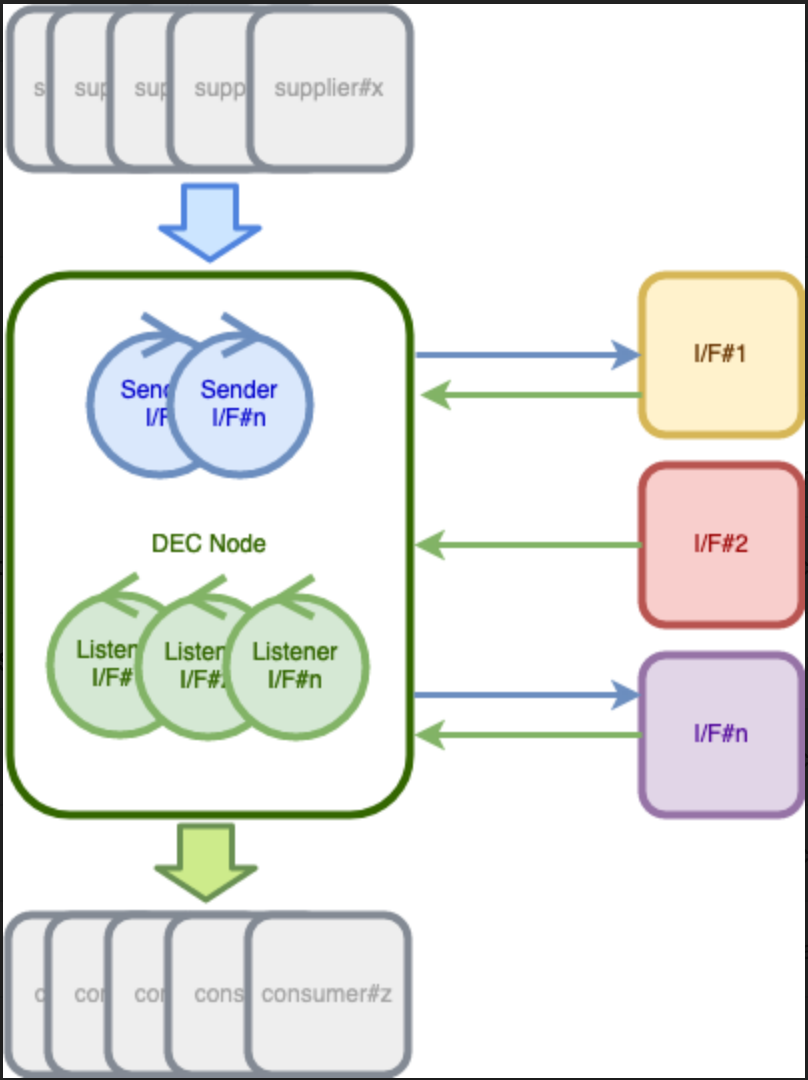
\includegraphics[scale=0.5]{DEC_Context_Diagram.png}
\end{figure}

\section{Definitions}
This section addresses a high level overview for the main design drivers that allows DEC to interface efficiently for the configured exchanges:

\begin{itemize}
	\item \textit{Circulation} : this term generally refers to any exchange of files either for retrieval upon \textit{pull} from or for distribution upon \textit{push} to any configured interface.
	\item \textit{Dissemination} : this term refers to the file-system local distribution into the Intray(s) of the files previously downloaded from a given interface as part of a \textit{pull} circulation.
	\item \textit{Download} : this term is used to refer to the actual retrieval of file from a given interface during a \textit{pull} iteration.
	\item \textit{Intray} : the final destination directory for downloaded files upon complete dissemination according to the rules.
	\item \textit{Pull} : this term refers to the circulation operation for filtering and listing up to the actual download of files from a given interface according to the configured rules. 
	\item \textit{Push} : this term refers to the circulation operation to upload the available file(s) in some interface. 
	\item \textit{Rule} : this generic term refers to the configuration items for \textit{pull} files, \textit{disseminate} them, and \textit{push} them.
\end{itemize}

\section{Design Drivers}
This section enumerates a high level overview for the main design drivers that allows DEC to interface efficiently for the configured exchanges:

\begin{itemize}
	\item \textit{Automation} : the ability to perform unattended autonomous circulation operations
	\item \textit{Flexibility} : the ability to \textit{pull} \& \textit{push} files from configurable interfaces and configurable circulation rules
	\item \textit{Robustness} : this is to perform “atomic” operations during file circulation ; the state for each operation is always known being network errors tolerant
	\item \textit{Performance} : parallelisation of the circulation to fruit the available network bandwidth, support of file compression mechanisms to reduce the footprint of transfers and local disseminations for which duplication of files by \textit{cp} or \textit{mv} can be avoided by usage of \textit{hardlinks}
	\item \textit{Resiliency} : to \textit{autonomously} recover from network errors, downtime and eventual glitches and resume operations during every iteration.
	\item \textit{Zero-copy} : to avoid new copies in the file system during \textit{dissemination} circulations.	
\end{itemize}

\section{Download DEC SW}
This section contains the links to download the DEC SW and the \textit{Gemfile} with the definition of the \textit{gem} dependencies. It is necessary to be logged-in with your DEIMOS \textit{gmail} account to \textit{authorise} the download.

\par
\noindent

\begin{itemize}
	\item \href{https://drive.google.com/uc?export=download&id=18TAD2BAJpHzgBdZGf3W8KQZCY7SPpKbU}{\textit{Gemfile}} : file with the \textit{gem} dependencies 
	\item \href{https://drive.google.com/uc?export=download&id=1gieDRpDEBzKv5Xr0qwPvBz34RHphTnQq}{\textit{dec-stable.gem}} : DEC gem installer
	\item\href{https://drive.google.com/uc?export=download&id=1JBAnxdRwaPK8PmrxuRi3qea43NOPRJbK/view?usp=sharing}{\textit{dec\_test.bash}} : definition of the environment variables used by the unit tests for bash console 
	\item\href{https://drive.google.com/uc?export=download&id=1HHWOVxCZbY6Surv_kKyF5kGTy45CvUKl/view?usp=sharing}{\textit{dec\_test.env}} : definition of the environment variables used by the unit tests for docker container parametrisation
\end{itemize}

\end{document}

